\documentclass{beamer}
\usetheme{KUL}
\usepackage{multirow}
\usepackage{multicol}
\usepackage{tikz}
\usepackage{ulem}
\usepackage{siunitx}
\newcommand
\itemS{
\item[\textbf{\S}]}
\definecolor{darkgreen}{rgb}{0,0.598,0.199}
\usepackage{times} % set font on times new roman
\usepackage{eurosym} % package for Euro sign
\usepackage{lineno}   % package for line numbering
\usepackage{subcaption}  % this package enables one to put several
% figures next to each other
\usepackage{textcomp}
\usepackage{setspace}
\usepackage{gensymb}
\usepackage{url}
\usepackage[backend=biber,style=numeric-comp,sorting=none]{biblatex}
\addbibresource{bib.bib}
\usepackage{hyperref} % this is for url links

%----------------------------------
% Fill in the essential Information
%----------------------------------

\title[Candlestick Patterns]{Performance of candlestick patterns on
intraday market data}
\subtitle{Thesis defence}
\author[W.\ Notermans]{Wout Notermans} % between [] is short name,
% between {} is long name
\date{July 27, 2025} % Here you can also just type something, e.g.
% October 10, 2017
\institute[KU Leuven]{Faculty of Science\\ Department of
Mathematics\\ Section of Statistics and Risk}

%----------------------------------
% ACTUAL PRESENTATION STARTS HERE
%----------------------------------

\begin{document}

% TITLE PAGE
{
  \setbeamertemplate{headline}{} %define local, empty header for title page
  \setbeamertemplate{footline}{} %define local, empty footer for title page
  \maketitle
}
\addtocounter{framenumber}{-1} % We don't count the title page

% \begin{kulblock}{Landslide}
%     A landslide is the downhill movement of soil mass
% \end{kulblock}

% ------------
% Introduction
% ------------

\section{Introduction}

\begin{frame}{Table of contents}
  \tableofcontents
\end{frame}

\begin{frame}[noframenumbering]{Table of contents}
  \tableofcontents[currentsection]
\end{frame}

\begin{frame}
  \begin{center}
    Can you predict what is going to happen on the stock market and make a profit based on these predictions?
  \end{center}
\end{frame}

\begin{frame}{Stock price \cite{berkshirehathaway}}
  \centering
  \includegraphics[width=0.8\textwidth]{Images/BRK.A_line.pdf}\\
\end{frame}

\begin{frame}{Candlestick construction}
  \centering
  \includegraphics[width=\textwidth]{Images/candlestick_construction.png}
  Construction of a candlestick \cite{chen2020}.
\end{frame}

\begin{frame}[noframenumbering]{Stock price \cite{berkshirehathaway}}
  \centering
  \includegraphics[width=0.8\textwidth]{Images/BRK.A_candle.pdf}
\end{frame}

\begin{frame}[noframenumbering]{Stock price \cite{berkshirehathaway}}
  \centering
  \includegraphics[width=0.8\textwidth]{Images/BRK.A_candlestick_pattern.pdf}
\end{frame}

\begin{frame}{Candlestick pattern examples}
  \centering
  \includegraphics[width=0.5\textwidth]{Images/risingthreemethods.pdf}%
  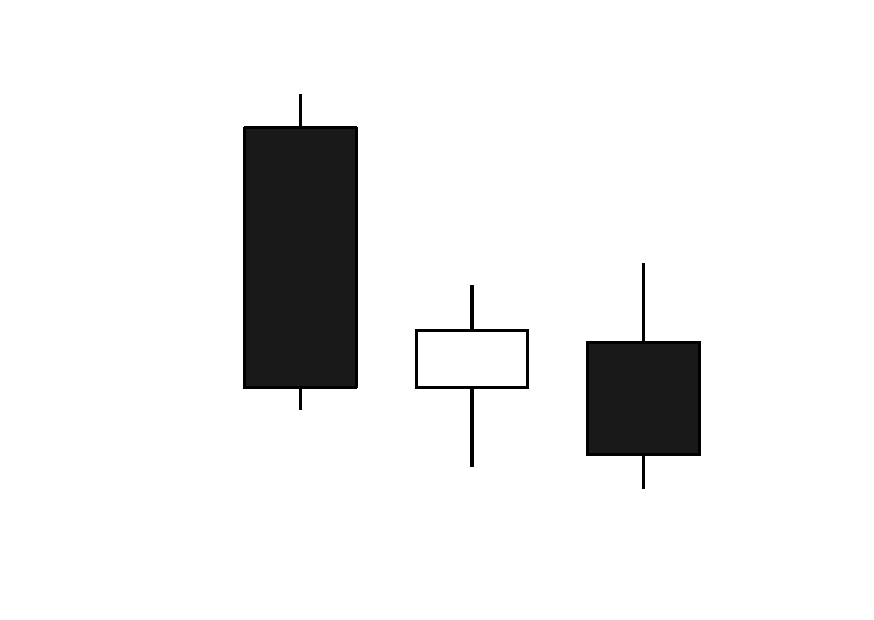
\includegraphics[width=0.5\textwidth]{Images/sticksandwich.pdf}
  ``Rising Three Methods'' and ``Stick Sandwich''
\end{frame}

\begin{frame}{History}
  \begin{itemize}
    \item Developed in the 1700s in Japan.
    \item Remained exclusive to the East until 1991.
    \item Has become a well-known technique, used by many traders.
  \end{itemize}
\end{frame}

\begin{frame}{Literature}
  \begin{itemize}
    \item Literature split between machine learning and rule based approach.
    \item Results are very split.
    \item Very few publications about intraday market data.
  \end{itemize}
\end{frame}

\begin{frame}
  \begin{kulblock}{Research question}
    Do candlestick patterns possess predictive power on\\
    intraday market data?
  \end{kulblock}
\end{frame}

% -----------
% Methodology
% -----------

\section{Methodology}

\begin{frame}[noframenumbering]{Table of contents}
  \tableofcontents[currentsection]
\end{frame}

\begin{frame}{Overview}
  \begin{itemize}
    \item Selection of data sets.
    \item Preprocessing of the data.
    \item Trends and technical indicators.
    \item Pattern detection.
    \item Pattern evaluation.
  \end{itemize}
\end{frame}

\begin{frame}{Data sets}
  \begin{itemize}
    \item BND: Bonds.
    \item GLD: Gold.
    \item QQQ: Stocks.
    \item SPY: Stocks.
    \item Geometric Brownian motion: Generated.
  \end{itemize}
\end{frame}

\begin{frame}{Preprocessing}
  \begin{itemize}
    \item Filter pre/after-market.
    \item Aggregation.
    \item Cross-validation to avoid bias and overfitting.
  \end{itemize}
\end{frame}

\begin{frame}{Preprocessing: calibration}
  \scalebox{0.8}{
    \begin{tabular}{cccccc}
      \hline
      & Doji & Short & Normal & Tall & Extremely tall \\
      Real body & $[0-10)$ & $[10-30)$ & $[30-70)$ & $[70-100]$ &  \\ \hline
      Shadow & $[0-10)$ & $[10-30)$ & $[30-70)$ & $[70-90)$ & $[90-100]$ \\ \hline
    \end{tabular}
  }
  \centering\\[1em]
  Percentiles of real bodies and shadows \cite{etschberger2006}.\\
  \includegraphics[width=0.5\textwidth]{Images/matching_low.pdf}
\end{frame}

\begin{frame}{Preprocessing: calibration}
  \begin{itemize}
    \item Assumes length and color candle independent.
    \item Has to be checked $\rightarrow$ Kolmogorov-Smirnov test.
      $$H_0: W = B \qquad H_1: W \neq B.$$
    \item Reject at 5\% significance.
  \end{itemize}
\end{frame}

\begin{frame}{Trend}
  \begin{itemize}
    \item Many patterns are only valid when the correct trend is present.
    \item Multiple ways of defining the trend in the literature.
    \item Example: count in/decreases in the moving average.
  \end{itemize}
\end{frame}

\begin{frame}{Pattern detection}
  \begin{itemize}
    \item Patterns are vaguely defined at best: a rigid classification is necessary.
    \item The paper ``A formal approach to candlestick pattern classification in financial time series'' does exactly this \cite{hu2019}.
    \item Define 103 candlestick patterns with strict conditions.
    \item Multiple comparisons problem addressed through Benjamini-Yekutieli.
  \end{itemize}
\end{frame}

\begin{frame}{Pattern detection: example}
  \centering
  \includegraphics[width=0.75\textwidth]{Images/mathold.pdf}\\
  ``Mat Hold''
\end{frame}

\begin{frame}{Pattern detection: prediction}
  \begin{itemize}
    \item Typically classified as buy/sell signal.
    \item Look at the results themselves instead of the predictions.
  \end{itemize}
\end{frame}

\begin{frame}{Pattern evaluation: stop-loss/take-profit}
  \begin{itemize}
    \item Buy after pattern is detected.
    \item Make use of stop loss/take profit margins.
    \item These are based on the ATR technical indicator so they scale with market activity.
  \end{itemize}
\end{frame}

\begin{frame}[noframenumbering]{Pattern evaluation: stop-loss/take-profit}
  \begin{itemize}
    \item This gives us a winning rate $\hat{\pi}$.
    \item Obtain a ``null win rate'' $\hat{\pi_0}$ through random sampling.
    \item Test significance with binomial test. \\ $$H_0:\hat{\pi}=\hat{\pi_0}\qquad\qquad H_1:\hat{\pi}>\hat{\pi_0}$$
  \end{itemize}
\end{frame}

\begin{frame}{Pattern evaluation: profitability score}
  $$\text{Adjusted $z$-score}=\overbrace{\dfrac{\hat{\pi}-\hat{\pi_0}}{\sqrt{\dfrac{\hat{\pi_0}(1-\hat{\pi_0})}{n}}}}^{z\text{-test}}\cdot\overbrace{\ln(\min\{n,5000\})}^{\text{Frequency adjustment}}$$
  This encapsulates:
  \begin{enumerate}
    \item The number of detected patterns.
    \item The win rate.
    \item The significance.
  \end{enumerate}
\end{frame}

\begin{frame}{Pattern evaluation: excess return}
  \begin{enumerate}
    \item Also consider the ``excess return'' $\hat{\pi}-\hat{\pi_0}$
    \item Duvinage et al. estimate that at least $0.05\%$ is required to be economically viable \cite{duvinage2013}.
  \end{enumerate}
\end{frame}

% -------
% Results
% -------

\section{Results}

\begin{frame}[noframenumbering]{Table of contents}
  \tableofcontents[currentsection]
\end{frame}

\begin{frame}{Detection results}
  \begin{itemize}
    \item Not many ``gapping" patterns.
    \item Some patterns are rare due to stringent conditions.
  \end{itemize}
  \centering
  \includegraphics[width=0.5\textwidth]{Images/windowfalling.pdf}%
  \includegraphics[width=0.5\textwidth]{Images/eveningstar.pdf}
  ``Window, Falling'' and ``Evening Star''
\end{frame}

\begin{frame}{Evaluation results: significance}
  \begin{itemize}
    \item Significant patterns are found.
    \item More significant buy than sell signals.
    \item A lot of variance between data sets/asset types.
    \item Aggregation decreases significance and $z$-score, but not excess return.
    \item Profit margins too small to be economical.
  \end{itemize}
\end{frame}

\begin{frame}[noframenumbering]{Evaluation results: significance}
  \centering
  \includegraphics[width=0.8\textwidth]{Images/buy_signals_QQQ.pdf}
\end{frame}

\begin{frame}[noframenumbering]{Evaluation results: significance}
  \centering
  \includegraphics[width=0.8\textwidth]{Images/z_score_QQQ.pdf}
\end{frame}

\begin{frame}[noframenumbering]{Evaluation results: significance}
  \centering
  \includegraphics[width=0.8\textwidth]{Images/excess_QQQ.pdf}
\end{frame}

\begin{frame}{Evaluation results: time of day}
  \begin{itemize}
    \item Entire day.
    \item One hour after open/before close.
    \item One hour after New York open.
    \item Limit to maximum 5 minutes.
  \end{itemize}
\end{frame}

\begin{frame}[noframenumbering]{Evaluation results: time of day}
  \centering
  \includegraphics[width=0.8\textwidth]{Images/z_score_time_BND.pdf}
\end{frame}

\begin{frame}[noframenumbering]{Evaluation results: time of day}
  \centering
  \includegraphics[width=0.8\textwidth]{Images/z_score_time_GLD.pdf}
\end{frame}

\begin{frame}{Evaluation results: little/no effect}
  \begin{itemize}
    \item Trend inclusion.
    \item Trend defining methods.
  \end{itemize}
\end{frame}

% ----------
% Conclusion
% ----------

\section{Conclusion and further research}

\begin{frame}[noframenumbering]{Table of contents}
  \tableofcontents[currentsection]
\end{frame}

\begin{frame}
  \begin{kulblock}{Research question}
    Do candlestick patterns possess any predictive power on intraday market data?
  \end{kulblock}
\end{frame}

\begin{frame}{Conclusion}
  \begin{itemize}
    \item Some patterns do appear to possess significant predictive power.
    \item Typically not consistent.
    \item This mainly holds true for buy signals.
    \item There is a lot of variance to these results.
    \item Not profitable enough to be economically viable.
  \end{itemize}
\end{frame}

\begin{frame}{Further research}
  \begin{itemize}
    \item Machine learning-based approach to detection/evaluation.
    \item Adapting definitions of patterns to market conditions.
    \item Tick-based candlesticks.
    \item Many alternative methods to define trends and to evaluate performance.
  \end{itemize}
\end{frame}

% ------------
% Bibliography
% ------------

\section*{Bibliography}

\begin{frame}[noframenumbering,allowframebreaks]
  \printbibliography
\end{frame}

\section*{}

\begin{frame}
  \begin{center}
    \color{cyan} \LARGE Questions?
  \end{center}
\end{frame}

\end{document}
